%-------------------------------------------------------------------------------
% seq64_qt_portmidi
%-------------------------------------------------------------------------------
%
% \file        seq64_qt_portmidi.tex
% \library     Documents
% \author      Chris Ahlstrom
% \date        2018-05-28
% \update      2018-08-25
% \version     $Revision$
% \license     $XPC_GPL_LICENSE$
%
%     Provides a discussion of the Qt5 GUI and portmidi, along with a Windows
%     implementation that Sequencer64 supports.
%
%-------------------------------------------------------------------------------

\section{Sequencer64 Qt5/PortMidi}
\label{sec:qt_portmidi}

   With version 0.95.1 of \textsl{Sequencer64}, we now provides builds using
   the \textsl{Qt 5} GUI framework and a heavily modified version of the
   PortMidi framework.
   With this additional work, we now have
   \index{Windows}
   \index{Sequencer64 for Windows}
   \index{qpseq64.exe}
   \textsl{Sequencer64 for Windows}.

   Currently, the Qt 5 user-interface is fundamentally the same as
   the \textsl{Kepler34} project (\cite{kepler34}).
   But it uses the internal functions of \textsl{Sequencer64} and adds a few
   features not yet present in \textsl{Kepler34}.
   It uses a tabbed interface, and slightly different ways of handling the main
   window (the "Live" tab), the performance window (the "Song" tab), and the
   editing window (the "Edit" tab).

   There is still a little amount of \textsl{Sequencer64} functionality that
   the Qt5/PortMidi version lacks:

   \begin{enumerate}
      \item No support for the special coloring of empty pattern slots
         or the pattern currently being edited.
      \item A reduced-functionality options/preferences dialog, lacking an
         editor for keystroke commands.
      \item Keystroke support is not as comprehensive as the Linux version.
      \item No support yet for variset or multi-wid.  What we will probably
         implement is variset and allow for any number of external live frames
         so that an arbitrary number of sets (banks) can be shown at once,
         each in its own window.
   \end{enumerate}

   We are incorporating existing \textsl{Sequencer64} user-interface
   features into this Qt5/PortMidi version as time and bug-fixes allow.

   With version 0.95.1, we have improved the Qt/Windows version by adding the
   following features:

   \begin{enumerate}
      \item An external pattern editor has been added that pretty much matches
         the standard \textsl{Sequencer64} pattern editor.  The tabbed
         pattern editor is still in place, but, due to space considerations,
         it will never support all of the features of the external window.
      \item The LFO (low-frequency oscillator) window now exists, and it can be
         called up from the external pattern editor.
      \item The external pattern editor supports background sequences, chord
         entry, event merging and extension, scales, snap, etc.
      \item The song editor has been improved, and also made available as an
         external window.
      \item The pattern and song editors now have better support for zooming
         via keystrokes.
   \end{enumerate}
   Some ill-advised features from \textsl{Sequencer64} will not be migrated.
   Ultimately, we want to replace the Gtkmm-2.4 user-interface completely.
   But this is awhile down the road.

   There are a number of alternate versions of \textsl{Sequencer64} using
   PortMidi:

   \begin{enumerate}
      \item A Gtkmm-2.4 user interface and PortMidi.  This version is
         Linux-only, and is useful for debugging the internal PortMidi code
         without worrying about the Qt5 user interface.
      \item A Qt 5 user interface and PortMidi on Linux.  This version is
         useful for people who like to experiment, and for debugging Qt5 and
         PortMidi issues at the same time.
      \item A Qt 5 user interface and PortMidi on Windows.  This version is
         basically working, but takes some special setup.
         See \sectionref{subsec:qt_portmidi_windows_setup} for details.
   \end{enumerate}

   We also have code in place to support
   \index{Mac OSX}
   \textsl{Mac OSX},
   but currently have no OSX system on which to build and test this
   code.  HELP WANTED!

   In the following sections, we cover the basic differences between the
   Gtkmm-2.4 and Qt 5 versions of the application, as well as how to set up
   \textsl{Sequencer64 for Windows}.

   We will not show all of the user interface elements, but we will mention
   some differences one will find.

\subsection{The Qt 5 User Interface}
\label{subsec:qt_portmidi_qt5_user_interface}

   \textsl{This section is out-of-date; many upgrades were made for version
   0.95.1.  And there is more to come.  Once we get it all finalized, we will
   update this section and its screen-shots.}

   The Qt5/PortMidi version of \textsl{Sequencer64} has an executable name of
   \texttt{qpseq64} (Linux) or \texttt{qpseq64.exe} (Windows).
   To keep explanations simple, we will refer to the Qt5/PortMidi version of
   \textsl{Sequencer64} as \textbf{qpseq64}.
   The Gtkmm-2.4/RtMidi version (Linux only) will be referred to as
   \textbf{seq64}.

   Here is a screenshot of the main user interface of \textsl{qpseq64}, with
   some of the patterns colored for emphasis.

\begin{figure}[H]
   \centering 
   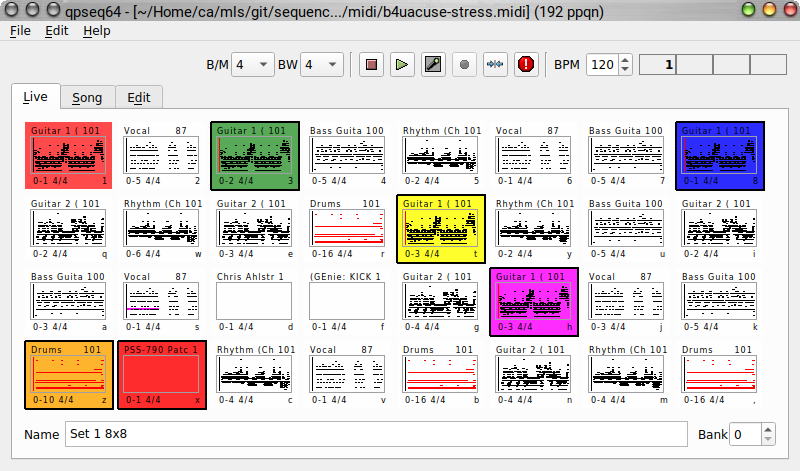
\includegraphics[scale=0.75]{kepler34/qt5-main-window-linux.png}
   \caption{Qt 5 Main Window, Linux}
   \label{fig:qt5_main_window_linux}
\end{figure}

   Note the difference in layout from the Gtkmm-2.4 version.
   Also notice that a number of controls from the Gtkmm version are missing.
   Some of these missing item will ultimately be added.

   Here is a similar screenshot in Windows 10.

\begin{figure}[H]
   \centering 
   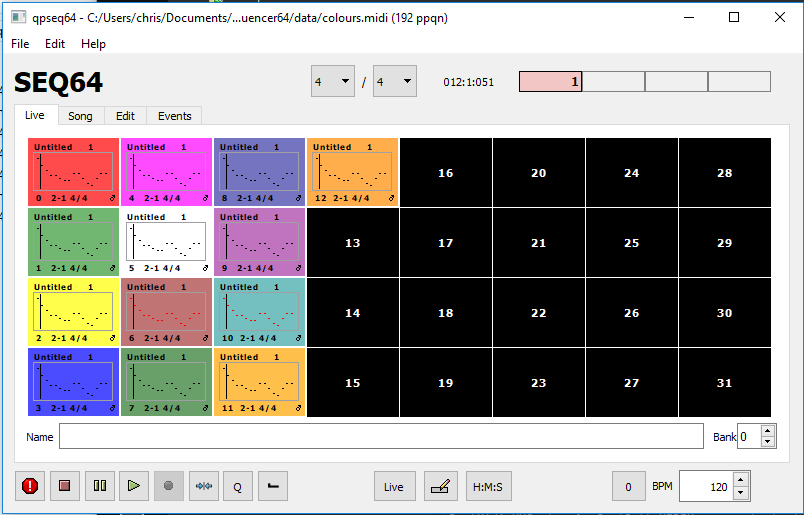
\includegraphics[scale=0.75]{kepler34/qt5-main-window-windows.png}
   \caption{Qt 5 Main Window, Windows 10}
   \label{fig:qt5_main_window_windows}
\end{figure}

   Coding an application for both Windows and Linux is very instructive, and
   often improves the overall code significantly.

\subsubsection{Qt 5 Live Tab}
\label{subsubsec:qt_portmidi_qt5_live_tab}

   The \textbf{Live} tab of \textsl{qpseq64}, as shown above, is very similar
   to the \textsl{seq64} version.  However, it currently doesn't support the
   varisets mode and the alternate row-by-column sizes of \textsl{seq64}.
   Additional features will be added as time goes on.

   The size of this window can be changed to a certain degree via
   the command-line option \texttt{--option scale=x.y}, where \texttt{x.y} can
   range from 0.4 to 3.0.  This can be made permanent via the
   \texttt{window-scale} setting in the "usr" file.

   In fact, all of the tabs except for the Events tab will expand properly to
   use additional space if the application is resized.

   In the future, we will likely provide external windows so that the user can
   view and work with a number of set/banks at the same time.

\subsubsection{Qt 5 Song Tab}
\label{subsubsec:qt_portmidi_qt5_song_tab}

\begin{figure}[H]
   \centering 
   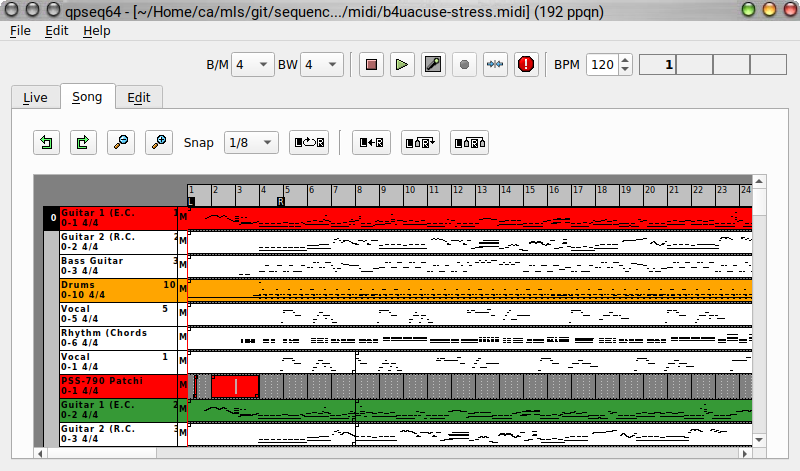
\includegraphics[scale=0.75]{kepler34/qt5-song-window-linux.png}
   \caption{Qt 5 Song Window, Linux}
   \label{fig:qt5_song_window_linux}
\end{figure}

   This window is very similar to the \textsl{seq64} version.
   Additional features may be added as time goes on.  In addition,
   this frame can be opened in its own external window by
   pressing the "Song Editor" button at the bottom of the main window.

\subsubsection{Qt 5 Edit Tab}
\label{subsubsec:qt_portmidi_qt5_edit_tab}

\begin{figure}[H]
   \centering 
   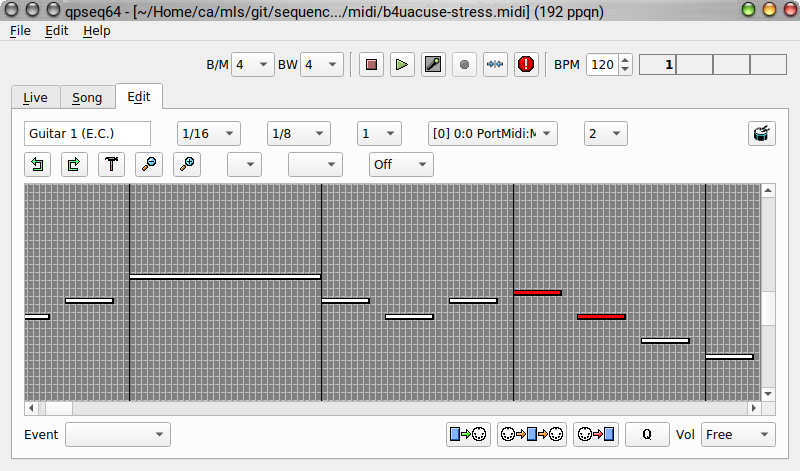
\includegraphics[scale=0.75]{kepler34/qt5-edit-window-linux.png}
   \caption{Qt 5 Edit Window, Linux}
   \label{fig:qt5_edit_window_linux}
\end{figure}

   This version of the pattern editor is a bit behind
   \textsl{seq64} for features, and currently looks more like the Gtkmm-2.4
   version.

   In addition, note that the event-data editor panel is not visible here.
   One must scroll down to the bottom of the window to see it and use it.
   Also note that that the \textbf{LFO} window is not accessible here.
   Finally, note that the note heights and vertical grid spacing are
   modifiable via

   With version 0.95.1, the pattern/slot popup menu has an option to open the
   pattern in an external window that has a lot more features than the
   pattern editor in the tab.  It also has a different scrolling mechanism,
   more like that of \textsl{seq64}.
   Note that only one of the tab/external pattern
   editors can be shown at the same time for a given pattern.
   This pattern editor is pretty much identical to the Gtkmm-2.4 version,
   except that it does not provide a "fruity" mode of mouse usage.

\subsubsection{Qt 5 Events Tab}
\label{subsubsec:qt_portmidi_qt5_events_tab}

\begin{figure}[H]
   \centering 
   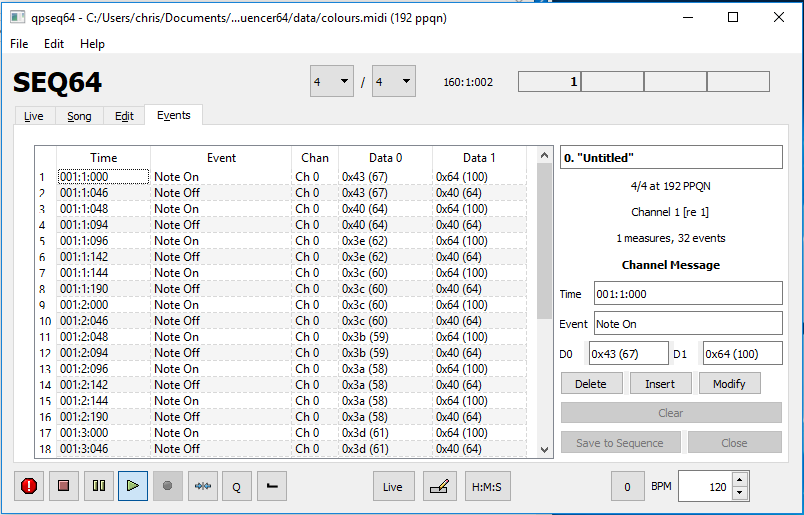
\includegraphics[scale=0.75]{kepler34/qt5-event-editor.png}
   \caption{Qt 5 Events Window}
   \label{fig:qt5_events_window}
\end{figure}

This window works a lot like
\sectionref{sec:seq64_event_editor}; please see that section for user
instructions.
Please remember that, at the present time, this view is meant
only for viewing events and making minor tweaks to a pattern, such
as eliminating problematic events.  It is not intended to be a full-featured
event editor.  In particular, note that editing within each cell in the event
table is not supported.  Event editing must be done in the right panel.
An event must be explicitly selected by clicking on it, before it can be
modified or deleted.

Also, if one adds or modifies an event to show up an the end of the pattern,
by modifying the time stamp, the event will appear there, but the
user-interface will remain at the current event.

\subsubsection{Qt 5 Edit / Preferences}
\label{subsubsec:qt_portmidi_qt5_edit_prefs}

\begin{figure}[H]
   \centering 
   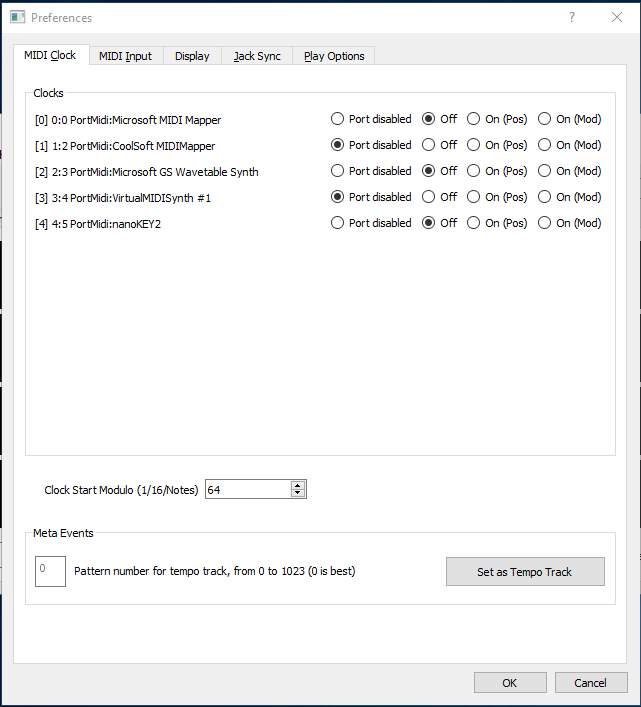
\includegraphics[scale=0.75]{kepler34/qt5-prefs-clock-windows.png}
   \caption{Qt 5 Clock Preferences, Windows}
   \label{fig:qt5_prefs_clock_windows}
\end{figure}

   In a newer version of this document, we will show the other preferences
   tabs.  There are many tabs we still need to add to this dialog.

   In particular, be sure to go to the \textbf{MIDI Input} tab and
   make sure that your desired input device (e.g. a MIDI keyboard) are shown
   and are enabled.

   Since the Qt GUI pretty much hardwires the keystrokes used for various
   functions such as muting and queuing, we might not provided a keystroke
   mapping editor.  To be determined.

   In any event, many of the keystrokes configured in the "rc" file are
   supported, but one might have to edit the "rc" file directly, keeping
   in mind that it uses Gtkmm-2.4 conventions for keystrokes.

\subsection{Sequencer64 Windows Setup}
\label{subsec:qt_portmidi_windows_setup}

   \textsl{Sequencer64 for Windows} (\textsl{qpseq64}) can be installed
   as a portable Zip package anywhere the user desires.  The package is
   self-contained, and contains all the the DLLs needed to run the program.
   \textsl{qpseq64} can also be installed via an NSIS-based installer,
   currently \texttt{sequencer64\_setup\_0.95.0-0.exe}.

\subsubsection{Sequencer64 Windows Issues}
\label{subsubsec:qt_portmidi_windows_setup_issues}

    When first starting \textsl{qpseq64} on \textsl{Windows}, one might
    experience some issues.  One issue is that the \textsl{Microsoft MIDI
    Mapper}, rumored to be removed in \textsl{Windows 8} and beyond, is still
    detected by the internal PortMidi library used in \textsl{qpseq64}.
    Another issue is that the built-in \textsl{Microsoft} wave-table
    synthesizer might not be accessible.

    We installed the
    \textsl{CoolSoft MIDIMapper} (\cite{midimapper}) and
    \textsl{VirtualMIDISYnth} (\cite{midisynth}) to try to get
    around these issues, and tried to turn off the
    \texttt{Windows System Sound} setup of
    \textsl{"Allow applications to restrict access to this device."}
    But we still had
    inaccessible devices, and the resulting errors would cause
    \textsl{qpseq64} to
    abort.  So we had to spend a lot of time adding support for
    the disabling of
    inaccessible ports, and saving and restoring the "rc" setup properly
    in the face of device-access errors.

    Here is some output logging on our Windows, generated using the
    \texttt{qpseq64} command-line option
    \texttt{-o log=virtualmidi.log},
    which dumps the log file into
    \texttt{C:/Users/chris/AppData/Local/sequencer64/virtualmidi.log}:

\begin{verbatim}
   qpseq64 
   C:/Users/chris/AppData/Local/sequencer64/virtualmidi.log 
   2018-05-13 09:06:58 
   [MIDIMAPPER] 'mapper in : midiInGetDevCaps() error for device 'MIDIMAPPER':
      'The specified device identifier is out of range'
   pm_winmm_general_inputs(): no input devices
   PortMidi MMSystem 0: Microsoft MIDI Mapper output opened
   PortMidi MMSystem 1: CoolSoft MIDIMapper output closed
   PortMidi MMSystem 2: Microsoft GS Wavetable Synth output opened
   PortMidi MMSystem 3: VirtualMIDISynth #1 output closed
   [Opened MIDI file,
      'C:/Users/chris/Documents/Home/sequencer64/data/b4uacuse-gm-patchless.midi']
   [Writing rc configuration C:/Users/chris/AppData/Local/sequencer64/qpseq64.rc]
   PortMidi call failed: [-1] 'Bad pointer'
   PortMidi call failed: [-1] 'Bad pointer'
   Begin closing open devices...
   Warning: devices were left open. They have been closed.
\end{verbatim}

    We still have some minor issues at start up and at exit, but are now able
    to play a tune on the wavetable synthesizer using the
    \texttt{--bus 2} option, which forces output to PortMidi buss 2,
    "Microsoft GS Wavetable Synth".

\subsubsection{Sequencer64 Windows Configuration Files}
\label{subsubsec:qt_portmidi_windows_setup_config}

    When you first run \textsl{qpseq64}
    on \textsl{Windows}, it will create a new configuration
    file, with inaccessible devices denoted in the
    \texttt{[midi-clock]} section of
    \texttt{C:/Users/username/AppData/Local/sequencer64/qpseq64.rc}
    by a \texttt{-1} value.

    On \textsl{Linux},
    the normal directory location of the \textsl{Sequencer64} configuration
    files is
    \texttt{/home/username/.config/sequencer64}.  There are various
    configuration file names, depending on the name of the built application:

\begin{verbatim}
        sequencer64.rc      The RtMidi Native ALSA/JACK version.
        sequencer64.usr     The same, but for user-interface settings.
        seq64portmidi.rc    The PortMidi Gtkmm 2.4 version.
        seq64portmidi.usr   The same, but for user-interface settings.
        qpseq64.rc          The PortMidi Qt 5 version.
        qpseq64.usr         The same, but for user-interface settings.
\end{verbatim}

    On \textsl{Windows},
    the conventional location is different, and the location used
    is \textsl{C:/Users/username/AppData/Local/sequencer64}.
    The files are:

\begin{verbatim}
        qpseq64.rc          The PortMidi Qt 5 version for Windows.
        qpseq64.usr         The same, but for some user-interface settings.
\end{verbatim}

    Typical of \textsl{Microsoft}, access to the \texttt{AppData} directory
    is not obvious... "we cannot have users monkeying with the configuration".
    To access \texttt{AppData}, highlight the user-name directory
    (e.g. \texttt{C:/Users/chris}, then append
    "AppData" to the end of it.  Voila! It is now visible in
    \textsl{Windows Explorer}.
    It is a Windows thang.

    Then click on the \texttt{sequencer64} directory.
    Open \texttt{qplseq64.rc} and see what is in it (scroll down a bit):

\begin{verbatim}
    [midi-clock]

    2    # number of MIDI clocks/busses

    # Output buss name: [0] 0:0 PortMidi:Microsoft MIDI Mapper
    0 0  # buss number, clock status

    # Output buss name: [2] 1:1 PortMidi:Microsoft GS Wavetable Synth (virtual)
    1 0  # buss number, clock status

    # Output buss name: [3] 1:1 PortMidi:nanoKEY2
    2 0  # buss number, clock status
    
    [midi-input]
    
    1    # number of input MIDI busses

	 # The first number is the port number, and the second number
	 # indicates whether it is disabled (0), or enabled (1).

	 # [1] 0:1 PortMidi:nanoKEY2
	 0 1
\end{verbatim}

   These settings can be accessed via
   \textbf{Edit / Preferences / MIDI Clock} and
   \textbf{Edit / Preferences / MIDI Input} to
	alter the ports accessible, in the \textsl{Windows}
   version of \textsl{Sequencer64}.
   The operating system may have some devices locked out, though.

   Generally, the device needs to have a "System Sound" setting that allows an
   application to grab exclusive access to the device.
   For now, do a web search for this error message:

\begin{verbatim}
   'The specified device is already in use.  Wait until it is free, and then
   try again.'
\end{verbatim}

%-------------------------------------------------------------------------------
% vim: ts=3 sw=3 et ft=tex
%-------------------------------------------------------------------------------
